\documentclass[12pt, letterpaper]{article}

% Packages
\usepackage[utf8]{inputenc}
\usepackage{geometry}
\usepackage{graphicx}
\usepackage{listings}
\usepackage{xcolor}
\usepackage{float}
\usepackage{enumitem}
\usepackage{array}
\usepackage{amsmath}
\usepackage{tikz}
\usepackage{hyperref}

\usetikzlibrary{positioning}

% Page Layout
\geometry{margin=1in}

% Code listing style
\definecolor{codebg}{rgb}{0.95,0.95,0.95}
\definecolor{codegreen}{rgb}{0,0.5,0}
\definecolor{codegray}{rgb}{0.5,0.5,0.5}
\definecolor{codepurple}{rgb}{0.58,0,0.82}

\lstdefinestyle{pythonstyle}{
    backgroundcolor=\color{codebg},
    commentstyle=\color{codegreen},
    keywordstyle=\color{blue},
    numberstyle=\tiny\color{codegray},
    stringstyle=\color{codepurple},
    basicstyle=\ttfamily\scriptsize,
    breakatwhitespace=false,
    breaklines=true,
    captionpos=b,
    keepspaces=true,
    numbers=left,
    numbersep=5pt,
    showspaces=false,
    showstringspaces=false,
    showtabs=false,
    tabsize=4,
    language=Python,
    frame=single,
}

\lstdefinestyle{outputstyle}{
    basicstyle=\ttfamily\tiny,
    breaklines=true,
    frame=single,
    numbers=none,
    backgroundcolor=\color{codebg},
    xleftmargin=0.5em,
    framexleftmargin=0.3em,
    aboveskip=0.5em,
    belowskip=0.5em,
}

% TikZ styles
\tikzset{
    netnode/.style={
        circle, draw, fill=white,
        minimum size=10mm, font=\bfseries,
        line width=0.6pt
    },
    edgelabel/.style={
        font=\small, fill=white, inner sep=2pt
    }
}

% Header Information
\title{\textbf{Homework 7}}
\author{Yousef Alaa Awad}
\date{\today}

% Custom Formatting Commands
\newcommand{\lab}[1]{\section*{Lab #1}}
\newcommand{\task}[1]{\subsection*{Task #1}}
\newcommand{\question}[1]{\noindent\textbf{Question: }#1\par\vspace{0.5em}}
\newcommand{\answer}{\noindent\textbf{Answer:}\par\vspace{0.5em}}

\begin{document}

\maketitle

% ============================================================================
% Q1
% ============================================================================
\section*{Q1 (10 pts)}

In Chapter 5-2, slide 12 (corresponding to Section 6.3 in textbook), we provided an outline of the derivation of the efficiency of slotted ALOHA. In this problem we'll complete the derivation.

\question{a. Recall that when there are $N$ active nodes, the efficiency of slotted ALOHA is $Np(1-p)^{N-1}$. Find the value of $p$ that maximizes this expression.}

\answer
Let $E(p) = Np(1-p)^{N-1}$. To find the maximum efficiency, we take the derivative of $E(p)$ with respect to $p$ and set it to zero:
\begin{align*}
\frac{dE}{dp} &= N(1-p)^{N-1} + Np(N-1)(1-p)^{N-2}(-1) \\
&= N(1-p)^{N-2} \left[ (1-p) - p(N-1) \right] \\
&= N(1-p)^{N-2} \left[ 1 - p - Np + p \right] \\
&= N(1-p)^{N-2} \left[ 1 - Np \right]
\end{align*}
Setting $1 - Np = 0$, we find:
\begin{equation*}
p = \frac{1}{N}
\end{equation*}

\question{b. Using the value of $p$ found in (a), find the efficiency of slotted ALOHA by letting $N$ approach infinity. Hint: $(1-1/N)^N$ approaches $1/e$ as $N$ approaches infinity.}

\answer
Using $p = 1/N$, the efficiency expression becomes:
\begin{equation*}
E = N\left(\frac{1}{N}\right)\left(1 - \frac{1}{N}\right)^{N-1} = \left(1 - \frac{1}{N}\right)^{N-1}
\end{equation*}
This can be rewritten as:
\begin{equation*}
E = \frac{(1 - 1/N)^N}{1 - 1/N}
\end{equation*}
As $N \to \infty$:
\begin{itemize}
    \item $(1 - 1/N)^N \to 1/e$
    \item $1 - 1/N \to 1$
\end{itemize}
Thus, the maximum efficiency as $N$ approaches infinity is:
\begin{equation*}
E \to \frac{1/e}{1} = \mathbf{\frac{1}{e}} \approx 0.368
\end{equation*}

% ============================================================================
% Q2
% ============================================================================
\section*{Q2 (15 pts)}

Suppose four active nodes---nodes A, B, C and D---are competing for access to a channel using slotted ALOHA. Assume each node has an infinite number of packets to send. Each node attempts to transmit in each slot with probability $p$. The first slot is numbered slot 1, the second slot is numbered slot 2, and so on.

\question{a. What is the probability that node A succeeds for the first time in slot 5?}

\answer
For node A to succeed for the first time in slot 5, it must fail to succeed in slots 1, 2, 3, and 4, and then succeed in slot 5.
\begin{itemize}
    \item Probability that node A succeeds in a given slot is $P_A = p(1-p)^3$.
    \item Probability that node A fails to succeed in a given slot is $1 - P_A = 1 - p(1-p)^3$.
\end{itemize}
Therefore, the probability is:
\begin{equation*}
P = \left(1 - p(1-p)^3\right)^4 \cdot p(1-p)^3
\end{equation*}

\question{b. What is the probability that some node (either A, B, C or D) succeeds in slot 4?}

\answer
The probability that any given node succeeds in a slot is $p(1-p)^3$. Since successes of different nodes in the same slot are mutually exclusive events, the probability that \textit{some} node succeeds is the sum of their individual success probabilities:
\begin{equation*}
P = 4p(1-p)^3
\end{equation*}

\question{c. What is the probability that the first success occurs in slot 3?}

\answer
For the first success to occur in slot 3, no node can succeed in slots 1 and 2, and some node must succeed in slot 3.
\begin{itemize}
    \item Probability of success in a slot = $4p(1-p)^3$.
    \item Probability of no success in a slot = $1 - 4p(1-p)^3$.
\end{itemize}
Therefore, the probability is:
\begin{equation*}
P = \left(1 - 4p(1-p)^3\right)^2 \cdot 4p(1-p)^3
\end{equation*}

\question{d. What is the efficiency of this four-node system?}

\answer
The efficiency is the probability of a successful transmission in a given slot, which we found in part (b):
\begin{equation*}
\text{Efficiency} = 4p(1-p)^3
\end{equation*}

% ============================================================================
% Q3
% ============================================================================
\section*{Q3 (15 pts)}

Consider the Figure below. MAC addresses and IP addresses have been provided on the right side. Suppose Host A sends a datagram to Host F.

\begin{figure}[H]
    \centering
    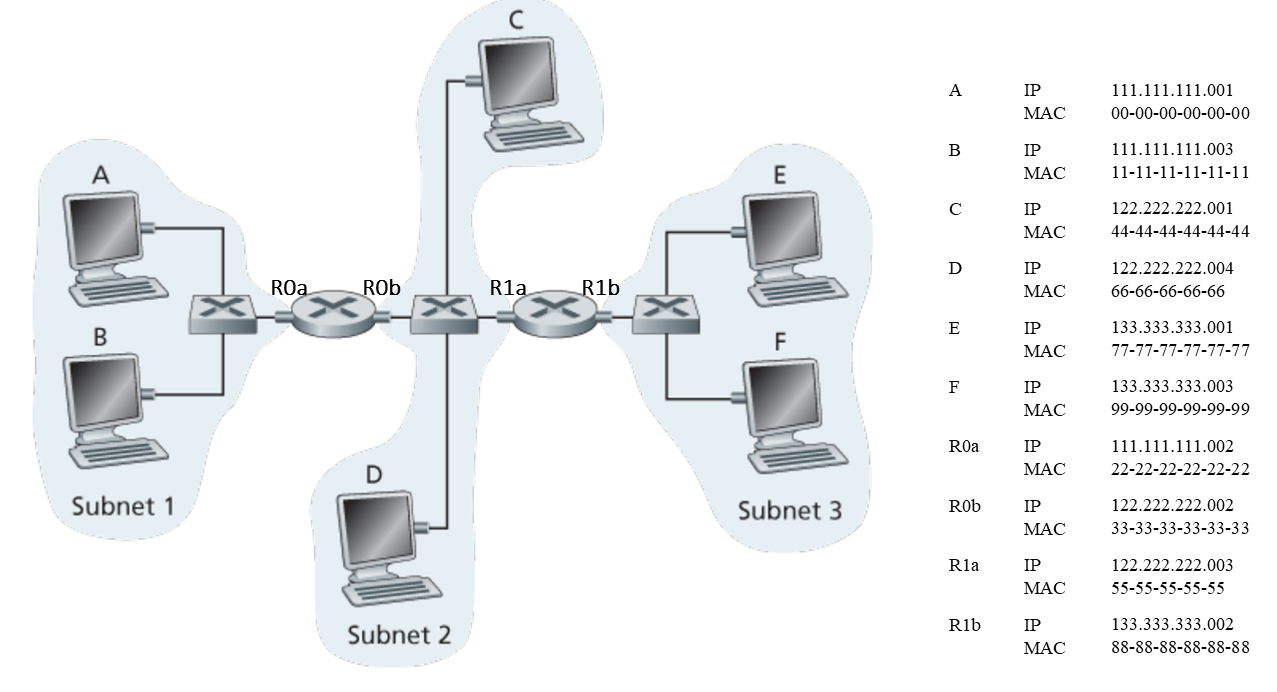
\includegraphics[width=0.9\textwidth]{image1.png}
\end{figure}

\question{a. Give the source and destination MAC addresses in the frame encapsulating this IP datagram as the frame is transmitted (i) from A to the left router, (ii) from the left router to the right router, (iii) from the right router to F. Also give the source and destination IP addresses in the IP datagram encapsulated within the frame at each of these points in time.}

\answer
The IP addresses remain unchanged from source to destination, while the MAC addresses change at each hop.
\begin{itemize}
    \item \textbf{(i) From A to Left Router (R0):}
    \begin{itemize}
        \item Source MAC: \texttt{00-00-00-00-00-00} (Host A)
        \item Dest MAC: \texttt{22-22-22-22-22-22} (R0a interface)
        \item Source IP: \texttt{111.111.111.001} (Host A)
        \item Dest IP: \texttt{133.333.333.003} (Host F)
    \end{itemize}
    \item \textbf{(ii) From Left Router (R0) to Right Router (R1):}
    \begin{itemize}
        \item Source MAC: \texttt{33-33-33-33-33-33} (R0b interface)
        \item Dest MAC: \texttt{55-55-55-55-55-55} (R1a interface)
        \item Source IP: \texttt{111.111.111.001} (Host A)
        \item Dest IP: \texttt{133.333.333.003} (Host F)
    \end{itemize}
    \item \textbf{(iii) From Right Router (R1) to Host F:}
    \begin{itemize}
        \item Source MAC: \texttt{88-88-88-88-88-88} (R1b interface)
        \item Dest MAC: \texttt{99-99-99-99-99-99} (Host F)
        \item Source IP: \texttt{111.111.111.001} (Host A)
        \item Dest IP: \texttt{133.333.333.003} (Host F)
    \end{itemize}
\end{itemize}

\question{b. Suppose now that the leftmost router in the Figure is replaced by a switch. Hosts A, B, C, and D and the right router are all star-connected into this switch. Give the source and destination MAC addresses in the frame encapsulating this IP datagram as the frame is transmitted (i) from A to the switch, (ii) from the switch to the right router, (iii) from the right router to F. Also give the source and destination IP addresses in the IP datagram encapsulated within the frame at each of these points in time.}

\answer
With the leftmost router replaced by a switch, Host A is in the same subnet as the left interface of the Right Router (R1a). The switch only forwards frames at the link layer, so it does not change MAC addresses.
\begin{itemize}
    \item \textbf{(i) From A to the Switch:}
    \begin{itemize}
        \item Source MAC: \texttt{00-00-00-00-00-00} (Host A)
        \item Dest MAC: \texttt{55-55-55-55-55-55} (R1a interface - default gateway)
        \item Source IP: \texttt{111.111.111.001} (Host A)
        \item Dest IP: \texttt{133.333.333.003} (Host F)
    \end{itemize}
    \item \textbf{(ii) From the Switch to Right Router (R1):}
    \begin{itemize}
        \item Source MAC: \texttt{00-00-00-00-00-00} (Host A)
        \item Dest MAC: \texttt{55-55-55-55-55-55} (R1a interface - default gateway)
        \item Source IP: \texttt{111.111.111.001} (Host A)
        \item Dest IP: \texttt{133.333.333.003} (Host F)
    \end{itemize}
    \item \textbf{(iii) From Right Router (R1) to Host F:}
    \begin{itemize}
        \item Source MAC: \texttt{88-88-88-88-88-88} (R1b interface)
        \item Dest MAC: \texttt{99-99-99-99-99-99} (Host F)
        \item Source IP: \texttt{111.111.111.001} (Host A)
        \item Dest IP: \texttt{133.333.333.003} (Host F)
    \end{itemize}
\end{itemize}

% ============================================================================
% Q4
% ============================================================================
\section*{Q4 (10 pts)}

\question{Short Answer: Suppose two nodes start to transmit at the same time a packet of length $L$ over a broadcast channel of rate $R$. Denote the propagation delay between the two nodes as $d_{prop}$. Will there be a collision if $d_{prop} < L/R$? Why or why not?}

\answer
\textbf{Yes}, there will be a collision. If two nodes start to transmit exactly at the same time, their signals will propagate towards each other and overlap on the channel, regardless of the relative values of $d_{prop}$ and $L/R$. The condition $d_{prop} < L/R$ merely ensures that each node is still transmitting its packet when the other node's signal arrives, which allows them to \textit{detect} the collision (as in CSMA/CD). Even if $d_{prop} \geq L/R$, a collision still occurs on the wire, but the transmitting nodes might not detect it before finishing their transmission.

\question{In CSMA/CD, after the fifth collision, what is the probability that a node chooses $K=4$? The result $K=4$ corresponds to a delay of how many seconds on a 10 Mbps Ethernet?}

\answer
\begin{itemize}
    \item After the 5th collision ($n=5$), the node chooses $K$ randomly from $\{0, 1, 2, \dots, 2^5-1\} = \{0, 1, \dots, 31\}$. Since there are 32 possible values and each is equally likely, the probability of choosing $K=4$ is $\mathbf{1/32}$ or $\mathbf{0.03125}$.
    \item For a 10 Mbps Ethernet, the base backoff time (slot time) is 512 bit times. 
    \begin{equation*}
    \text{Slot Time} = \frac{512 \text{ bits}}{10 \times 10^6 \text{ bps}} = 51.2 \mu s
    \end{equation*}
    If $K=4$, the delay is $4 \times 51.2 \mu s = 204.8 \mu s = \mathbf{0.0002048 \text{ seconds}}$.
\end{itemize}

\question{How big is the MAC address space? The IPv4 address space? The IPv6 address space?}

\answer
\begin{itemize}
    \item \textbf{MAC address space:} 48 bits long, so there are $2^{48}$ possible addresses ($\approx 2.81 \times 10^{14}$).
    \item \textbf{IPv4 address space:} 32 bits long, so there are $2^{32}$ possible addresses ($\approx 4.29 \times 10^9$).
    \item \textbf{IPv6 address space:} 128 bits long, so there are $2^{128}$ possible addresses ($\approx 3.40 \times 10^{38}$).
\end{itemize}

\end{document}